\pdfoutput=1
\documentclass[aps,prl,twocolumn,showpacs,superscriptaddress,nofootinbib,reprint]{revtex4-2}

% --- Packages
\usepackage{amsmath,amssymb,amsfonts,mathtools}
\usepackage{array}
\usepackage{graphicx}
\usepackage{bm}
\usepackage{siunitx}
\usepackage[hidelinks]{hyperref}
\usepackage[nameinlink,capitalise]{cleveref}
\usepackage{microtype}
\usepackage{xspace}
\usepackage{bm}
\sisetup{separate-uncertainty=true}
\allowdisplaybreaks
\usepackage{tikz}
\usepackage{pgfplots} \pgfplotsset{compat=1.18}
\usetikzlibrary{positioning}
\usepackage{booktabs}

% avoid conflicts with physics/amsmath
\let\dd\relax\let\abs\relax\let\norm\relax\let\braket\relax\let\vev\relax\let\tr\relax\let\order\relax
\let\matrix\relax

% ==============================
% GAGE Macros (MS-bar@MZ default)
% ==============================

% ------- Global toggles -------
\newif\ifPRLBoxes   \PRLBoxestrue
\newif\ifUseSI      \UseSIfalse     % default: natural units (G = Ω / m_p^2)
\newcommand{\maybeBox}[1]{\ifPRLBoxes\boxed{#1}\else#1\fi}

% ---------- Constants ----------
\providecommand{\GN}{G_{\mathrm N}}
\providecommand{\MPl}{M_{\rm P}}          % reduced Planck mass
\providecommand{\Mp}{m_p}
\providecommand{\hbarc}{\hbar c}

% ---------- Scales ----------
\providecommand{\MZ}{M_Z}
\providecommand{\Mstar}{M_\ast}

% ---------- Gauge couplings (hats = MS-bar@MZ) ----------
\providecommand{\alphas}{\hat{\alpha}_s}
\providecommand{\alphaTwo}{\hat{\alpha}_2}
\providecommand{\alphae}{\hat{\alpha}}
\providecommand{\alphaGpp}{\alpha^{(\mathrm{pp})}_{G}}

% ---------- Integer projection / depth ----------
\providecommand{\chis}{\boldsymbol{\chi}}         % (16,13,2)
\providecommand{\Psivec}{\hat{\boldsymbol{\Psi}}} % (ln hats)
\providecommand{\XiDepth}{\hat{\Xi}}              % \hat\Xi = \chi·\hat\Psi
\providecommand{\XiEq}{\hat{\Xi}^{(\mathrm{eq})}}
\providecommand{\DXi}{\Delta\hat{\Xi}}

% ---------- Gate ----------
\DeclareRobustCommand{\PiGate}[1]{\Pi\!\left(#1\right)}
\providecommand{\sigchi}{\sigma_{\chi}}
\providecommand{\Gstar}{G_\ast}                   % equilibrium coupling (SM-only)
\providecommand{\Gx}{\Gstar\,\PiGate{\XiDepth}}
\let\Gate\PiGate

% ---------- Field-space metric ----------
\providecommand{\Kfs}{\mathbf{K}(\Psivec)}
\providecommand{\Keq}{\mathbf{K}_{\rm eq}}
\DeclareRobustCommand{\normK}[1]{\ensuremath{\left\lVert#1\right\rVert_{\Keq}}}

% ---------- Derived canonicals ----------
\providecommand{\Lchi}{\Lambda_\chi}

% ---------- Math utils ----------
\providecommand{\LN}{\ln}
\providecommand{\dd}{\mathrm{d}}
\newcommand{\vev}[1]{\langle #1\rangle}
\DeclareMathOperator{\tr}{tr}
\providecommand{\abs}[1]{\ensuremath{\lvert#1\rvert}}
\providecommand{\norm}[1]{\ensuremath{\lVert#1\rVert}}
\providecommand{\order}[1]{\ensuremath{\mathcal{O}(#1)}}
\providecommand{\MSbar}{\overline{\mathrm{MS}}}

% ---------- Invariant (plain Ω) ----------
% Use Ω directly in text/math; no subscripted variant needed.

% ---------- Display boxes ----------
\newcommand{\OmegaProdBox}{\maybeBox{\ensuremath{%
  \Omega \;=\; \hat\alpha_s^{16}\,\hat\alpha_2^{13}\,\hat\alpha^{2}}}}
\newcommand{\GfromOmegaNat}{\maybeBox{\ensuremath{%
  G \;=\; \dfrac{\Omega}{m_p^{2}}}}}
\newcommand{\GfromOmegaSI}{\maybeBox{\ensuremath{%
  G \;=\; \dfrac{\hbar c}{m_p^{2}}\,\Omega}}}
\newcommand{\GfromOmegaCompact}{\maybeBox{\ensuremath{%
  G \;=\; \dfrac{\Omega\,\hbar c}{m_p^{2}}}}}
\newcommand{\GEquilBox}{\ifUseSI\GfromOmegaSI\else\GfromOmegaNat\fi}

% ---------- Lichnerowicz ----------
\providecommand{\DeltaL}{\Delta_{\!L}}

% ---------- Canonical ΔG/G ----------
\providecommand{\FracDG}{\ensuremath{\frac{\Delta G}{G}}}

% ---------- Gate + lab-null boxes ----------
\newcommand{\GateBox}{\maybeBox{\ensuremath{%
  \frac{\Gx}{\Gstar} \;=\; \PiGate{\XiDepth}
  \;=\; \exp\!\Big[-\frac{(\XiDepth-\XiEq)^2}{\sigchi^2}\Big]}}}
\newcommand{\ParityNullBox}{\maybeBox{\ensuremath{%
  \FracDG\;\simeq\;\frac{\DXi^2}{\sigchi^2}\quad
  (\Pi'(\XiEq)=0,\; G(x)=\Gstar\,\Pi(\Xi))}}}

% ---------- Soft-mode scalar ----------
\providecommand{\phiChi}{\phi_{\chis}}
\newcommand{\ParityNullPhiBox}{\maybeBox{\ensuremath{%
  \FracDG\;\simeq\;\frac{\phiChi^{2}}{\Lchi^{2}}\quad
  (\phi_{\chis}=\chis^{\!\top}(\Psivec-\vev{\Psivec})/\normK{\chis},\;
  \Lchi=\sigchi/\normK{\chis})}}}

% ==== Helpers for normalization & one-line boxes ====
\providecommand{\sXi}{s_{\Xi}} % s_Xi = ΔXi/σχ
\newcommand{\DefTriplet}{\ensuremath{%
  \sXi\equiv\DXi/\sigchi,\;
  \phiChi\equiv\DXi/\normK{\chis},\;
  \Lchi\equiv\sigchi/\normK{\chis}}}
\newcommand{\LabNull}{\ensuremath{%
  \FracDG=\sXi^{2}=(\phiChi/\Lchi)^{2}}}

% ---------- SI units (optional) ----------
\DeclareSIUnit{\eV}{eV}
\DeclareSIUnit{\MeV}{MeV}
\DeclareSIUnit{\GeV}{GeV}
\DeclareSIUnit{\fm}{fm}

% ---------- Safe PRL box macro ----------
\newcommand{\prlbox}[1]{%
  \noindent\begingroup
  \setlength{\fboxsep}{6pt}%
  \fbox{\begin{minipage}{0.96\columnwidth}\raggedright #1\end{minipage}}%
  \endgroup
}


\begin{document}

\title{Gauge-Aligned Gravity Emergence (GAGE): SM-derived gravitational coupling $G(Q)$}
\author{Michael DeMasi, DNP}
\affiliation{Independent Researcher, Milford, CT 06460, USA}
\date{\today}

\begin{abstract}
Within the SM at $\mu=\MZ$ ($\MSbar$), a unique primitive projector $\chis=(16,13,2)$ defines the gauge–log depth $\Xi=\chis\!\cdot\!\Psivec$. An even curvature gate $\Pi(\Xi)=\exp[-(\Delta\Xi)^2/\sigma_\chi^2]$ with $\Pi'(\Xi_{\rm eq})=0$ yields a GR-normalized, massless tensor sector ($m_{\mathrm{PF}}=0$) and $G(x)=G(\MZ)\Pi(\Xi(x))$, where $G(\MZ)=\hat\Omega(\MZ)\hbar c/m_p^2$ and $\hat\Omega=\hat\alpha_s^{16}\hat\alpha_2^{13}\hat\alpha^2$ (hats: $\MSbar$\ at $\mu=\MZ$). Two direct tests: (i) quadratic lab-null $\Delta G/G\simeq(\Delta\Xi/\sigma_\chi)^2$; (ii) closure/LOO with $\hat\Omega(\MZ)/\alpha_G^{(\mathrm{pp})}=1.09373393$ and $\hat\alpha_s^\star(\MZ)=0.1173411\pm1.86\times10^{-5}$. Inputs are SM-pinned; metrology is used only \emph{a posteriori}.
\end{abstract}

\maketitle


% ===== Section 1: Motivation + Premise + Alignment Principle =====

\paragraph*{Motivation.}
Despite its precision, the Standard Model has not yielded a self-contained derivation of Newton’s constant $G_N$ or a massless spin-2 graviton within its gauge structure. We propose an \emph{alignment principle}: near the electroweak scale, the gauge system aligns with the soft eigenmode of the equilibrium kinetic metric, enforcing parity-even curvature at the lab point. At $\mu=\MZ$ in $\MSbar$, the SNF-certified projector $\chis=(16,13,2)$ fixes the gauge–log depth $\Xi=\chis\!\cdot\!\Psivec$; an even gate $\Pi(\Xi)$ with $\Pi'(\Xi_{\rm eq})=0$ yields a GR-normalized, massless spin-2 sector with no new fields or tunable parameters and defines the emergent coupling $G$. The framework is parameter-free and falsifiable: with $\sXi\equiv\Delta\Xi/\sigma_\chi$, $\phi_\chi\equiv\Delta\Xi/\normK{\chis}$, and $\Lambda_\chi\equiv\sigma_\chi/\normK{\chis}$, one finds $\Delta G/G=\sXi^2=(\phi_\chi/\Lambda_\chi)^2$; closure is tested \emph{a posteriori} against metrology via $\alpha_G^{(\mathrm{pp})}=G_N m_p^2/(\hbar c)$.

\paragraph*{Premise.}
Work in logarithmic coupling space $\Psivec=(\ln\hat\alpha_s,\ln\hat\alpha_2,\ln\hat\alpha)$, where multiplicative renormalization becomes additive and basis transports are linear~\cite{Weinberg1996_QFTv2,PeskinSchroeder1995_QFT,Langacker2017_SMBeyond}. We seek a \emph{single}, basis-invariant scalar depth in this space that governs the curvature response and defines the emergent coupling $G(x)$. Its existence is not assumed but must arise from SM structure and be protected by a symmetry enforcing an even equilibrium response (\emph{i.e.}, a null first derivative).

\paragraph*{Alignment principle (physical motivation).}
Let $\Keq\!\succ\!0$ denote the equilibrium kinetic metric on $\Psivec$. 
Small variations organize along its \emph{soft eigenmode}—the direction of minimal kinetic curvature. 
We find numerically, using SM pins~\cite{PDG2024,PDG2025_GaugeHiggs}, that the gauge system aligns its response along this mode. 
Alignment has two immediate consequences: 
(i)~\textbf{Parity protection.} Near equilibrium, the response is even, so the leading deviation is quadratic in the depth displacement. The resulting \emph{parity-null} is directly testable—any observed linear term falsifies the mechanism. 
(ii)~\textbf{Tensor-sector normalization.} With even parity at the laboratory point, the linearized tensor dynamics coincide with GR (luminal helicity-2, no Pauli–Fierz mass). The graviton sector thus \emph{emerges} as the parity-even curvature response of the aligned gauge system~\cite{Carroll2004_SG,Will2014_LRR_TestsGR}. 

This alignment-first view provides the physical intuition before the algebra: the next sections identify the unique direction (certificate), define the depth $\Xi$, specify the even gate $\Pi(\Xi)$, derive the $\beta$-function for $G$, and establish closure and falsifiers. 

In Fisher-metric terms, alignment corresponds to motion along the soft eigenvector of $\Keq$—the direction of least informational curvature. Equivalently, systems minimize Fisher resistance by cohering along the soft mode, the information-geometry analog of least action.

\paragraph*{Integer certificate and depth.}
The alignment principle requires a single scalar coordinate in coupling space that remains invariant under renormalization–basis changes. From the one-loop decoupling lattice of the SM, the Smith normal form (SNF) isolates a unique primitive left-kernel generator~\cite{AppelquistCarazzone1975_Decoupling,KannanBachem1979_SNF,Newman1997_SNF},
\begin{align*}
\chis=(16,13,2),
\end{align*}
certifying that only one integer combination of gauge couplings remains invariant under one-loop decoupling transformations (Appelquist–Carazzone regime). This integer projector defines the gauge–log depth
\begin{align*}
\Xi=\chis\!\cdot\!\Psivec,\qquad
\Psivec=(\ln\hat\alpha_s,\ln\hat\alpha_2,\ln\hat\alpha),
\end{align*}
with local fluctuation $\Delta\Xi=\Xi-\Xi_{\rm eq}$. Log coordinates render multiplicative renormalization additive and basis transports linear~\cite{Weinberg1996_QFTv2,PeskinSchroeder1995_QFT}:
$\Psivec'=A\Psivec$, $\chis'=A^{-\top}\chis$, so $\Xi=\chis\!\cdot\!\Psivec$ is basis-invariant. Under metric transport $K'=A^{-\top}KA^{-1}$,
\begin{align*}
\|\chis\|_{K}^{2}=\chis^{\!\top}K\,\chis=\chis'^{\!\top}K'\chis',
\end{align*}
so both $\|\chis\|_{K}$ and the gate scale $\Lambda_\chi=\sigma_\chi/\|\chis\|_{K}$ remain invariant under basis choice. The integer certificate, scalar depth, and their transport properties complete the algebraic foundation for the curvature gate introduced next.
\medskip

\prlbox{%
\textbf{SNF certificate (sketch).}\;
$\Delta W_{\rm EM}=\begin{bmatrix}8&8&224\\[2pt]0&1&18\end{bmatrix}$ has integer rank~2, giving 
${\rm ker}_{\mathbb Z}(\Delta W_{\rm EM})=\mathrm{span}\{\pm\chi_{\rm EM}\}$ with 
$\chi_{\rm EM}=(-10,-18,1)$ and $\Delta W_{\rm EM}\chi_{\rm EM}=0$. 
Unimodular transport $M^{\!\top}\chi_{\rm EM}=\chis=(16,13,2)$ fixes the primitive generator, unique up to sign (full proof in SM~Sec.~S1).
}
\medskip

\paragraph*{Even gate and definition of $G(x)$.}
Having identified the invariant scalar depth $\Xi=\chis\!\cdot\!\Psivec$, we introduce the curvature-response function (the \emph{gate}) that modulates the emergent gravitational coupling. The gate must satisfy:  
(i)~even parity about equilibrium [$\Pi'(\Xi_{\rm eq})=0$];  
(ii)~analyticity and positivity for all $\Xi$;  
(iii)~normalization $\Pi(\Xi_{\rm eq})=1$ (recovering GR at equilibrium); and  
(iv)~minimal parameter freedom.  

A minimal analytic, even, and positive form satisfying these is the Gaussian gate
\begin{align*}
\Pi(\Xi)=\exp\!\Big[-\frac{(\Delta\Xi)^2}{\sigma_\chi^2}\Big],\qquad 
\Pi'(\Xi_{\rm eq})=0,\quad \Pi(\Xi_{\rm eq})=1,
\end{align*}
which enforces parity-even curvature modulation and smooth suppression beyond the Planck-thin envelope ($|\Delta\Xi|\!\sim\!\sigma_\chi$). With $\sXi\!=\!\Delta\Xi/\sigma_\chi$, $\phi_\chi\!=\!\Delta\Xi/\!\normK{\chis}$, and $\Lambda_\chi\!=\!\sigma_\chi/\!\normK{\chis}$, the laboratory null becomes $\Delta G/G=\sXi^2=(\phi_\chi/\Lambda_\chi)^2$. The width $\sigma_\chi$ is fixed by Fisher curvature from SM covariance at $\mu=\MZ$~\cite{PDG2024,PDG2024_EWReview,PDG2025_GaugeHiggs}, leaving no tunable parameters.

\textbf{Gate parity.}
If $\Pi$ is even and $C^2$ near $\Xi_{\rm eq}$, then $\Pi'(\Xi_{\rm eq})=0$ and $\Pi(\Xi_{\rm eq}+\Delta\Xi)=1-(\Delta\Xi)^2/\sigma_\chi^2+\order{(\Delta\Xi)^4}$; any $\order{(\Delta\Xi)}$ term falsifies parity or alignment. Writing the laboratory template as
\[
\frac{\Delta G}{G}=A\,s+B\,s^{2}+\order{s^{3}},\qquad
s\equiv\frac{\Delta\Xi}{\sigma_\chi},
\]
an even gate predicts $A=0$, $B=1$. Equivalently, in the $\phi_\chi$ normalization,
\[
\frac{\Delta G}{G}=A'\phi_\chi+B'\phi_\chi^{2}+\dots,\qquad
A'=0,\quad B'=1/\Lambda_\chi^{2}.
\]
Any reproducible odd term ($A\neq0$ or $A'\neq0$) falsifies alignment parity.

\paragraph*{Definition (natural units).}
In natural units ($\hbar=c=1$), the SM fixes the gravitational coupling via the dimensionless product
\begin{equation}
G \equiv \frac{\Omega}{m_p^{2}},\qquad 
\Omega \equiv \alpha_s^{16}\alpha_2^{13}\alpha^{2},\qquad 
G(x)=G\,\Pi(\Xi(x)). \label{eq:Gdef}
\end{equation}
For SI units, restore $\hbar c$:
\begin{equation}
G(\MZ)=\frac{\hat\Omega(\MZ)\,\hbar c}{m_p^{2}},\qquad 
\hat\Omega=\hat\alpha_s^{16}\hat\alpha_2^{13}\hat\alpha^{2}. \label{eq:GSI}
\end{equation}
\medskip

% Optional macro boxes (move to SM if space is tight)
\begin{minipage}{0.98\columnwidth}
\begin{center}
\OmegaProdBox \qquad
\GEquilBox \\[4pt]
\GateBox
\end{center}
\end{minipage}
\medskip

% ===== Figure: Even gate and quadratic parity-null =====
\begin{figure}[t]
\centering

% --- (A) Even gate Π(s) with s = ΔΞ/σχ ---
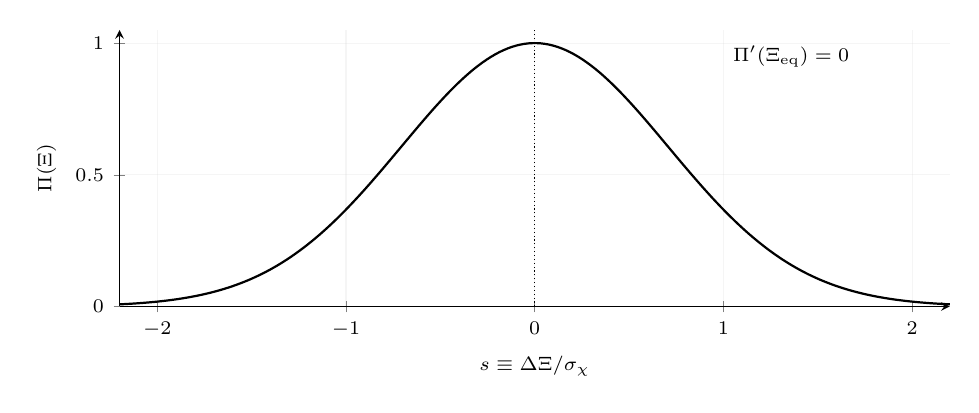
\begin{tikzpicture}
\begin{axis}[
  width=\columnwidth, height=0.42\columnwidth,
  xlabel={$s \equiv \Delta\Xi/\sigma_\chi$},
  ylabel={$\Pi(\Xi)$},
  xmin=-2.2, xmax=2.2, ymin=0, ymax=1.05,
  xtick={-2,-1,0,1,2}, ytick={0,0.5,1},
  tick label style={font=\scriptsize},
  label style={font=\scriptsize},
  domain=-2.2:2.2, samples=200,
  axis lines=left,
  grid=both, grid style={opacity=0.15}
]
  % Π(s) = exp(-s^2)
  \addplot[thick] {exp(-x^2)};
  % Mark equilibrium and note Π'(Ξ_eq)=0
  \addplot[densely dotted] coordinates {(0,0) (0,1.05)};
  \node[anchor=west,font=\scriptsize] at (axis cs:1.0,0.95) {$\Pi'(\Xi_{\rm eq})=0$};
\end{axis}
\end{tikzpicture}

\vspace{4pt}

% --- (B) Quadratic parity-null: ΔG/G vs s (shape with Λ_gate=1) ---
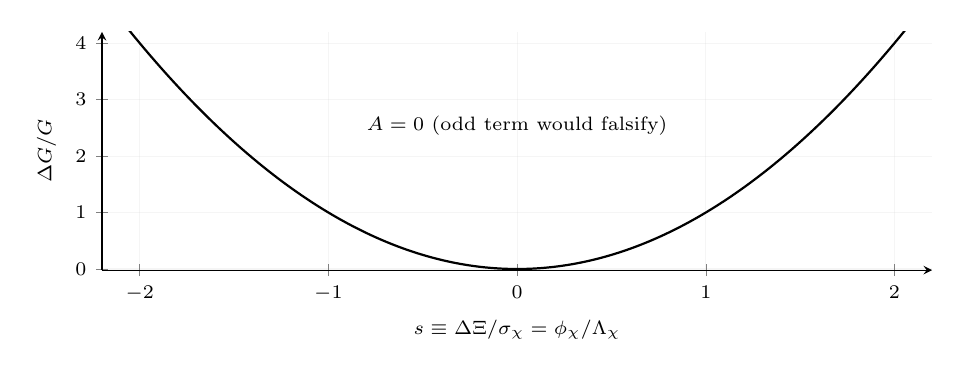
\begin{tikzpicture}
\begin{axis}[
  width=\columnwidth, height=0.38\columnwidth,
  xlabel={$s \equiv \Delta\Xi/\sigma_\chi = \phi_\chi/\Lambda_\chi$},
  ylabel={$\Delta G/G$},
  xmin=-2.2, xmax=2.2,
  ymin=-0.02, ymax=4.2,  % shape for Λ_gate=1 (y = s^2)
  xtick={-2,-1,0,1,2}, ytick={0,1,2,3,4},
  tick label style={font=\scriptsize},
  label style={font=\scriptsize},
  domain=-2.2:2.2, samples=200,
  axis lines=left,
  grid=both, grid style={opacity=0.15}
]
  % Template shape: ΔG/G = s^2 / Λ_gate^2 (Λ_gate=1 for visualization)
  \addplot[thick] {x^2};
  % Annotate odd-term falsifier
  \node[anchor=south,font=\scriptsize] at (axis cs:0,2.2) {$A=0$ (odd term would falsify)};
\end{axis}
\end{tikzpicture}

\caption{Even gate $\Pi(\Xi)=\exp[-(\Delta\Xi)^2/\sigma_\chi^2]$ vs $s=\Delta\Xi/\sigma_\chi$ with parity condition $\Pi'(\Xi_{\rm eq})=0$, enforcing the quadratic response $\Delta G/G\simeq(\Delta\Xi)^2/\sigma_\chi^2=\phi_\chi^2/\Lambda_\chi^2$. Any odd term $As$ would falsify alignment.}
\end{figure}


\paragraph*{Parity-even lab null and tensor sector.}
Even parity of the gate enforces a quadratic curvature response near equilibrium. 
With $\Keq\!\succ\!0$ and alignment of $\hat\chi=\chis/\normK{\chis}$ to the soft eigenvector of $\Keq$,
\begin{align}
\frac{\Delta G}{G}\simeq\frac{(\Delta\Xi)^2}{\sigma_\chi^2}
=\frac{\phi_\chi^2}{\Lambda_\chi^2},\qquad &
\phi_\chi=\frac{\chis^{\!\top}(\Psivec-\langle\Psivec\rangle)}{\normK{\chis}},\\
\Lambda_\chi=&\frac{\sigma_\chi}{\normK{\chis}}. \label{eq:labnull}
\end{align}
This constitutes the \emph{quadratic lab null}: any linear term in $\Delta G/G$ falsifies parity or alignment.

\medskip
\noindent\setlength{\fboxsep}{6pt}%
\fbox{%
  \begin{minipage}{0.96\columnwidth}\raggedright
  \textbf{No $h$–$\phi$ mixing at linear order.}\;
  $S\!\supset\!\tfrac{\MPl^2}{2}\Pi(\Xi)R$. 
  Since $\Pi'(\Xi_{\rm eq})=0$, the variation $\delta\Omega=\MPl^2\Pi'(\Xi_{\rm eq})\,\delta\Xi$ vanishes, removing the $(g_{\mu\nu}\Box-\nabla_\mu\nabla_\nu)\delta\Omega$ term at $\order{h}$. 
  The remaining equation $\mathcal{E}_{\mu\nu}^{\ \alpha\beta}h_{\alpha\beta}=0$ 
  is the Lichnerowicz operator with $m_{\mathrm{PF}}=0$.
  \end{minipage}%
}\par\vspace{3pt}
\medskip

Because $\Pi'(\Xi_{\rm eq})=0$, the linearized equation reduces to
\begin{equation}
\Delta_L h_{\mu\nu}\equiv -\Box h_{\mu\nu}=0, \label{eq:Lichnerowicz}
\end{equation}
so the tensor mode is GR-normalized, massless, and luminal (helicity-2)~\cite{Carroll2004_SG,Will2014_LRR_TestsGR,Cassini2003_PPN,LVK2021_TestsGR}.

\paragraph*{Pinned scales.}
With $K_{\rm eq}\!\succ\!0$, the gate scale is
\begin{equation}
\Lambda_\chi=\frac{\sigma_\chi}{\|\chi\|_{K_{\rm eq}}}. \label{eq:Lchi_def}
\end{equation}
From SM pins at $\mu=\MZ$ one finds $\sigma_\chi=247.683$ and $\|\chi\|_{K_{\rm eq}}=17.6278$, giving $\Lambda_\chi=14.0507$ (derivation in the Supplement).

\begin{table}[h]
\centering
\caption{Equilibrium kinetic metric $K_{\rm eq}$: eigenvalues and alignment diagnostics.}
\begin{tabular}{@{}lccc@{}}
\toprule
Eigenvalues $(\lambda_1,\lambda_2,\lambda_3)$ & $\|\chi\|_{K_{\rm eq}}$ & $\cos\theta_K$ & $\varepsilon_\chi$ \\
\midrule
(0.7243, 2.0156, 3.2599) & 17.6278 & 0.9999999998 & $<10^{-8}$ \\
\bottomrule
\end{tabular}
\end{table}

\paragraph*{Running of $G$ and Ward-flatness.}
Because $G$ is composed of SM couplings, its renormalization follows theirs. Differentiating $\Xi=\chis\!\cdot\!\Psivec$ gives
\[
\beta_{\Xi}\equiv \frac{d \Xi}{d\ln Q}
=16\frac{\beta_{\alpha_s}}{\alpha_s}
+13\frac{\beta_{\alpha_2}}{\alpha_2}
+2\frac{\beta_{\alpha}}{\alpha}=0\ \ 
\]\[
\text{(1 loop; Ward-flat)}. \label{eq:betaxi}
\]
Thus $\Xi$ and $G$ are stationary at one loop, avoiding basis artifacts~\cite{Weinberg1996_QFTv2,PeskinSchroeder1995_QFT}. Preregistered flatness windows and masks are evaluated in the SM; Fig.~\ref{fig:FQ} shows the monitor $F(Q)$ within bounds.

\begin{figure}[htbp]
\centering
\includegraphics[width=0.98\linewidth]{FQ_bounds.pdf}
\caption{Projected flatness monitor $F(Q)$ within preregistered electroweak and low-GeV windows. One-loop flatness corresponds to $\beta_\Xi=0$; mild threshold kinks appear outside the EW window.}
\label{fig:FQ}
\end{figure}

Beyond equilibrium, slow variation of $K_{\rm eq}$ produces adiabatic tracking of the soft mode (dynamic alignment) and a small two-loop drift (quantified in the Supplement).

The running of $G$ follows directly:
\begin{equation}
\beta_G\equiv \frac{d\ln G}{d\ln Q}
=16\frac{\beta_{\alpha_s}}{\alpha_s}
+13\frac{\beta_{\alpha_2}}{\alpha_2}
+2\frac{\beta_{\alpha}}{\alpha}
=0+O(\hat\alpha_i^{\,2}), \label{eq:betaG}
\end{equation}
so $G$ is flat at one loop with bounded higher-order drift~\cite{Jegerlehner2019_alphaRun}. Physically,
\begin{equation}
G(x)=G\,\Pi(\Xi(x)),\qquad
G=\frac{\Omega}{m_p^{2}}. \label{eq:Gphysrepeat}
\end{equation}
At $\mu=\MZ$ ($\MSbar$), comparison is made \emph{a posteriori} to the metrological coupling $\alpha_G^{(\mathrm{pp})}$~\cite{CODATA2022_RMP,PDG2024_PhysConstants}.

\paragraph*{Closure and prediction.}
The \emph{closure test} links the SM invariant to metrology:
\begin{equation}
\hat\Omega(\MZ)=\hat\alpha_s^{16}\hat\alpha_2^{13}\hat\alpha^2
\stackrel{?}{=}
\alpha_G^{(\mathrm{pp})}\equiv\frac{G_N m_p^2}{\hbar c}. \label{eq:closure}
\end{equation}
If equality holds within uncertainties,
\begin{equation}
G(\Xi_{\rm eq})=\frac{\hat\Omega(\MZ)\hbar c}{m_p^{2}}=G(\MZ). \label{eq:Geq}
\end{equation}
Inverting gives the leave-one-out (LOO) forecast,
\begin{equation}
\hat\alpha_s^{\star}(\MZ)
=\!\left[\frac{\alpha_G^{(\mathrm{pp})}}{\hat\alpha_2^{13}\hat\alpha^{2}}\right]^{1/16}
=0.1173411\pm1.86\times10^{-5}, \label{eq:LOO}
\end{equation}
consistent with the PDG mean ($-0.73\sigma$)~\cite{PDG2024,PDG2025_GaugeHiggs}. The closure ratio
\begin{equation}
\frac{\hat\Omega(\MZ)}{\alpha_G^{(\mathrm{pp})}}=1.09373393\quad(+9.37\%) \label{eq:closure_ratio}
\end{equation}
serves as the empirical benchmark~\cite{CODATA2022_RMP,PDG2024_PhysConstants,PDG2024,PDG2024_EWReview}.

\paragraph*{Matching (UV$\!\to\!$IR).}
Define the IR normalization via a dimensionless matching factor $Z_G$:
\begin{align}
G(\MZ)=\frac{\hat\Omega(\MZ)\,\hbar c}{m_p^{2}},\qquad
G_N\equiv Z_G\,G(\MZ),\\
Z_G=\frac{\alpha_G^{(\mathrm{pp})}}{\hat\Omega(\MZ)}
=0.91430\ (-8.57\%). \label{eq:matching}
\end{align}
This $Z_G$ absorbs scheme, threshold, and higher-order effects; the full budget is detailed in the Supplement.

\paragraph*{Helicity scale.}
At equilibrium, soft-mode alignment fixes
\begin{align}
&\Lambda_\chi=\frac{\sigma_\chi}{\|\chi\|_{K_{\rm eq}}}=14.0507\ (\approx14.05),\\
&\omega_{\rm hel}=\Lambda_\chi^{-1},\\
&T_{\rm hel}=2\pi\,\Lambda_\chi\simeq 88\,t_P. \label{eq:helicity}
\end{align}
This \emph{Planck-thin curvature envelope} sets the coherence length of the emergent tensor mode and bounds the quadratic response $\Delta G/G\simeq \phi_\chi^{2}/\Lambda_\chi^{2}$ (see SM Sec.~S8).

\paragraph*{Falsifiers (any suffices).}
The construction is parameter-free; any single failure falsifies it:
\begin{enumerate}
\item \textbf{Non-unique integer certificate.}
SNF must yield a unique primitive left-kernel generator $\chis=(16,13,2)$; any alternate integer solution of comparable norm breaks the projection symmetry~\cite{KannanBachem1979_SNF,Newman1997_SNF,AppelquistCarazzone1975_Decoupling}.

\item \textbf{Odd (linear) curvature response.}
With $\Pi'(\Xi_{\rm eq})=0$, a measured linear term $A s$ in
$\Delta G/G = A s + B s^2 + \dots$ (where $s=\Delta\Xi/\sigma_\chi$) contradicts the quadratic lab-null in Eq.~\eqref{eq:labnull}. 
\emph{Example (illustrative):} taking $s=9$ from SM pins gives
$\Delta G/G \simeq s^2 = (\phi_\chi/\Lambda_\chi)^2 = 1.32\times10^{-3}$,
accessible to symmetric $\pm s$ clock/torsion tests; fits must be consistent with $A=0$.

\item \textbf{Tensor-sector anomaly.}
Any Pauli–Fierz mass or non-luminal dispersion violates GR-normalized propagation (Eq.~\eqref{eq:Lichnerowicz})~\cite{Will2014_LRR_TestsGR,LVK2021_TestsGR,Cassini2003_PPN}.

\item \textbf{Metric instability or misalignment.}
$K_{\rm eq}\!\succ\!0$ with $\cos\theta_K\simeq1$ must hold; a negative eigenvalue or deviation beyond $\varepsilon_\chi$ signals ghost/locking failure (Table~1).

\item \textbf{Ward-flatness violation.}
The projected flow must satisfy $\beta_\Xi=0$ within preregistered EW and low-GeV masks (Eq.~\eqref{eq:betaxi}); significant drift implies RG-scheme dependence or breakdown of aligned projection~\cite{Weinberg1996_QFTv2,PeskinSchroeder1995_QFT}.

\item \textbf{Closure or LOO failure.}
Deviation of $\hat\Omega/\alpha_G^{(\mathrm{pp})}$ from unity beyond pinned uncertainties (Eq.~\eqref{eq:closure_ratio}), or $\hat\alpha_s^\star(\MZ)$ outside PDG bounds (Eq.~\eqref{eq:LOO}), falsifies identification of $G$ as SM-derived~\cite{CODATA2022_RMP,PDG2024,PDG2024_PhysConstants,PDG2025_GaugeHiggs}.
\end{enumerate}

\paragraph*{Implications.}
Gravity emerges as the parity-even curvature response of the Standard Model gauge sector, with
\[
G(x)=G(\MZ)\,\Pi(\Xi(x))
\]
fixed entirely by $\{\hat\alpha_s,\hat\alpha_2,\hat\alpha\}$ at $\mu=M_Z$~\cite{PDG2024,PDG2024_EWReview,PDG2025_GaugeHiggs,Carroll2004_SG}.
Two direct signatures make the framework falsifiable:
(i) the quadratic lab-null $\Delta G/G\simeq(\Delta\Xi/\sigma_\chi)^2$, and
(ii) the closure ratio $\hat\Omega/\alpha_G^{(\mathrm{pp})}=1.09373393$.
Any reproducible odd-parity term or closure mismatch beyond pinned uncertainties would refute the mechanism~\cite{Will2014_LRR_TestsGR,Cassini2003_PPN,LVK2021_TestsGR}.

The spurion-even gate and $\chi$-projection imply a conserved alignment current,
\begin{align}
J_\chi^\mu
  &= \Pi(\Xi)\,\chi^{\!\top}K_{\rm eq}\,\partial^\mu\hat\Psi, \nonumber\\[3pt]
\partial_\mu J_\chi^\mu
  &= 0 + \mathcal{O}\!\big((\Delta\Xi)^3,\text{2L drift},\varepsilon_\chi\big), \label{eq:align_current}
\end{align}
the Noether current associated with rigid depth shifts of $\Xi$ at equilibrium.
This conservation law is the gauge-depth analog of energy–momentum conservation under spacetime translations: alignment preserves curvature “energy’’ within the gauge sector.
Operationally, any reproducible odd (linear) response [$A\neq0$ in $\Delta G/G=A s+B s^2+\cdots$]
corresponds to $\partial_\mu J_\chi^\mu\neq0$ and thus falsifies alignment.

\paragraph*{Scope note.}
This Letter derives the gravitational coupling $G$ from SM couplings and demonstrates empirical closure. Dynamic tensor-sector extensions—including the helicity frequency, Planck-thin envelope, drift law, and the conserved alignment current—are detailed in the Supplemental Material. All analytic derivations and pinned numerical checks are reproducible from the accompanying \texttt{GAGE\_repo}. A companion study will extend the alignment–conservation framework to a fully dynamical formulation, developing the stress-energy, effective Lagrangian, geometric-fiber, informational, and temporal extensions that complete the GAGE description of gravity.

\begin{acknowledgments}
This work was conducted independently with no external funding. The author thanks the Particle Data Group (PDG), CODATA, Overleaf, and Python for open-access tools and data. An AI-assisted writing tool (OpenAI ChatGPT) was used for language editing and organizational assistance; all scientific content and responsibility rest with the author. The author declares no competing interests.
\end{acknowledgments}

\paragraph*{Data availability}
All data supporting this work (pins, equations, figure data, and scripts) are included in the Letter, the Supplemental Material, and the accompanying \texttt{GAGE\_repo}; additional materials are available from the author upon reasonable request.

\bibliographystyle{apsrev4-2}
\bibliography{gage_prl_refs}

\end{document}

